\documentclass[10pt,aspectratio=169]{beamer}

\usetheme{Madrid}
\usepackage[T1]{fontenc}
\usepackage[utf8]{inputenc}
\usepackage{amsmath,amssymb}
\usepackage{booktabs}
\usepackage{graphicx}
\usepackage{xcolor}

\definecolor{accent}{HTML}{2563EB}
\definecolor{accent2}{HTML}{DC2626}
\definecolor{accent3}{HTML}{059669}
\definecolor{good}{HTML}{059669}
\definecolor{bad}{HTML}{DC2626}

\setbeamercolor{frametitle}{bg=accent,fg=white}
\setbeamertemplate{itemize item}{\textcolor{accent}{$\bullet$}}
\setbeamertemplate{navigation symbols}{}
\setbeamertemplate{footline}[frame number]

\title{Time-Varying Covariates in Mortgage Survival}
\subtitle{Part E(ii) --- Andersen--Gill Cox Extension}
\author{Yueqi Lin}
\institute{MTH 9877 --- Baruch College, Spring 2026}
\date{May 13, 2026}

% =========================================================================
\begin{document}

% ---- Title ---------------------------------------------------------------
\begin{frame}[plain]
    \titlepage
\end{frame}

% ---- 1. Motivation -------------------------------------------------------
\begin{frame}{Static Cox discards the most important prepayment signal.}
    \begin{columns}[T,onlytextwidth]

        \column{0.50\textwidth}
        \begin{block}{Standard Cox (11 features)}
        \small\vspace{2pt}
        One row per loan; all covariates fixed at origination.
        Macro features captured as vintage-era snapshots.
        Cannot track rate cycles, burnout, or equity build
        after origination.
        \vspace{2pt}
        \end{block}

        \vspace{0.5em}

        \begin{block}{Andersen--Gill (13 features)}
        \small\vspace{2pt}
        One row per loan-month; $\mathbf{x}_i(t)$ updated each period.
        Extends the same static base with the four time-varying
        features, tracking the full path of rate incentive and
        equity. 100K loans $\times$ ${\sim}47$ months $= 4.68$M intervals.
        \vspace{2pt}
        \end{block}

        \column{0.46\textwidth}
        \vspace{0.2em}
        \small\textbf{Time-varying features} --- updated every month
        \vspace{0.4em}

        \begin{tabular}{@{}p{2.5cm}p{4.1cm}@{}}
            \toprule
            \textbf{Feature} & \textbf{What it captures} \\
            \midrule
            \addlinespace[2pt]
            \texttt{rate\_incentive} & $r_{\text{orig}}{-}r_{\text{mkt}}(t)$: live option value to refinance; tracks rate cycles and burnout \\
            \addlinespace[4pt]
            \texttt{ELTV}            & equity from amortisation and HPI gains; high ELTV suppresses refi \\
            \addlinespace[4pt]
            \texttt{unemployment}    & macro labour cycle; proxies Fed easing in high-unemp periods \\
            \addlinespace[4pt]
            \texttt{hpi\_yoy}        & home-price appreciation unlocking cash-out refinancing \\
            \addlinespace[2pt]
            \bottomrule
        \end{tabular}

    \end{columns}
\end{frame}

% ---- 2. Model ------------------------------------------------------------
\begin{frame}{The Andersen--Gill model estimates $\boldsymbol{\beta}$ from monthly risk comparisons.}

    \textbf{Hazard function} \quad (identical in form to standard Cox)
    \[
        h_i(t) \;=\; h_0(t)\,\exp\!\bigl(\boldsymbol{\beta}^\top \mathbf{x}_i(t)\bigr)
    \]
    \small
    $\mathbf{x}_i(t)$ is the \textbf{current} covariate vector, updated each month.
    $\boldsymbol{\beta}$ is a single coefficient vector estimated across all loan-months.

    \medskip
    \normalsize\textbf{Log partial likelihood} \quad (maximised to obtain $\hat{\boldsymbol{\beta}}$)
    \[
        \ell(\boldsymbol{\beta}) \;=\;
        \sum_{i:\,\delta_i=1}
        \Biggl[
            \underbrace{\boldsymbol{\beta}^\top \mathbf{x}_i(t_i)}_{\substack{\text{log-score of}\\\text{the prepaying loan}}}
            \;-\;\log
            \underbrace{\sum_{j \in \mathcal{R}(t_i)}
            \exp\!\bigl(\boldsymbol{\beta}^\top \mathbf{x}_j(t_i)\bigr)}_{\substack{\text{sum over all loan-months}\\\text{active at }t_i}}
        \Biggr]
    \]
    \small
    At each event: \textit{given a prepayment at $t_i$, what is the probability it was loan $i$
    rather than any other active loan?}
    Maximising $\ell$ estimates $\hat{\boldsymbol{\beta}}$ without specifying $h_0(t)$.

\end{frame}

% ---- 3. Feature trajectories ---------------------------------------------
\begin{frame}{Rate incentive and current LTV diverge sharply across vintages.}
    \begin{center}
        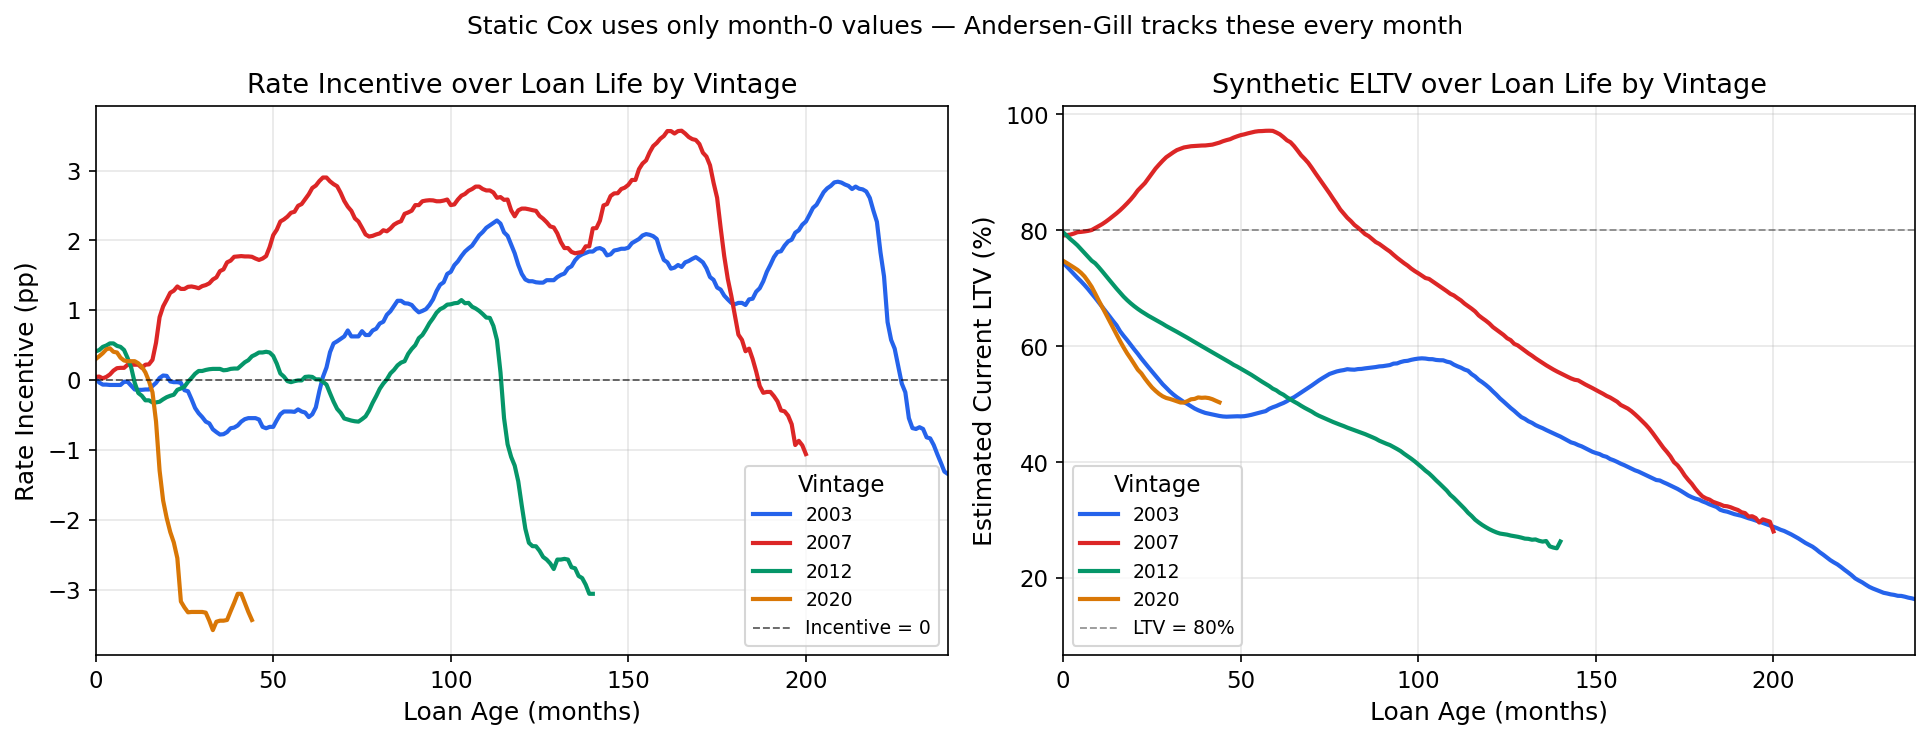
\includegraphics[width=0.90\linewidth]{processed/Eii_tv_feature_trajectories}
    \end{center}
    \vspace{-0.5em}
    \begin{center}
        \small
        Static Cox uses only month-0 values --- Andersen-Gill tracks these every month.
    \end{center}
\end{frame}

% ---- 4. Coefficient comparison -------------------------------------------
\begin{frame}{Live macro signals flip sign versus origination-era snapshots.}
    \begin{center}
        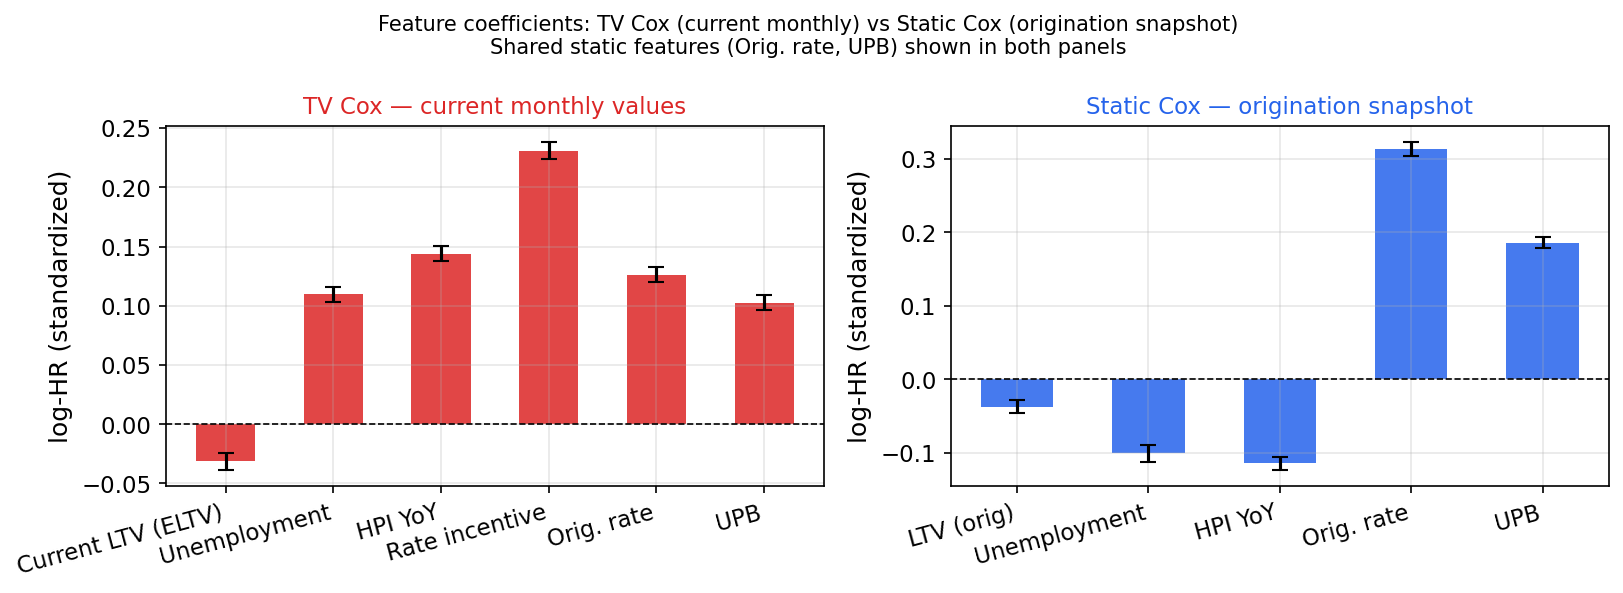
\includegraphics[width=0.92\linewidth]{processed/Eii_static_vs_tv}
    \end{center}
    \vspace{-0.3em}
    \small
    \begin{itemize}\itemsep2pt
        \item \texttt{rate\_incentive}: dominant positive predictor in TV Cox; near zero at origination, absent from Static Cox
        \item Macro signals (unemployment, HPI) flip sign --- vintage-era snapshots capture a different regime than monthly values
    \end{itemize}
\end{frame}

% ---- 5. Model performance ------------------------------------------------
\begin{frame}{TV Cox leads through $T=60$; static Cox overtakes at $T=84$--$T=120$.}
    \begin{columns}[c,onlytextwidth]
        \column{0.56\textwidth}
        \begin{center}
            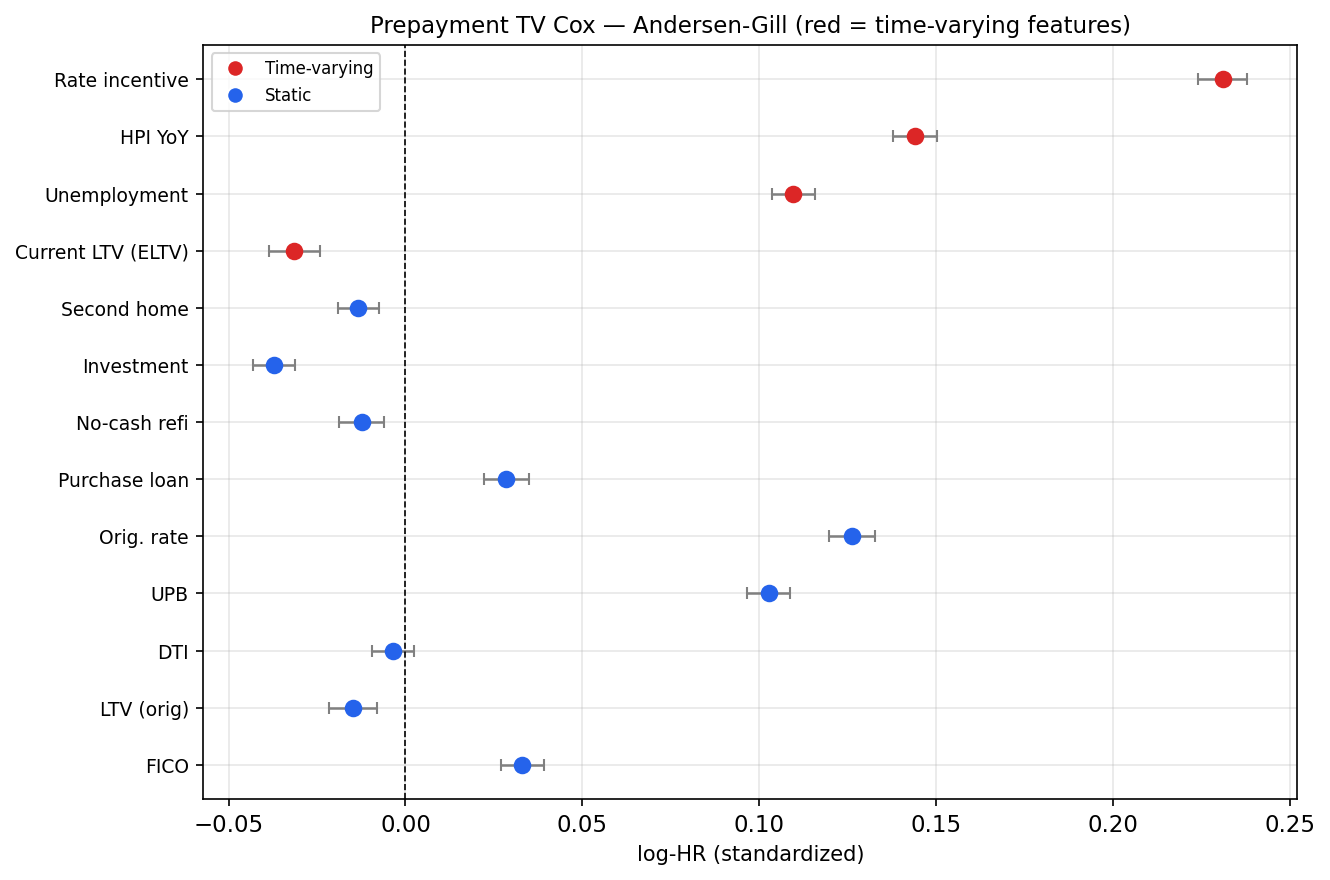
\includegraphics[width=\linewidth]{processed/Eii_tv_cox_forest}
        \end{center}

        \column{0.42\textwidth}
        \begin{center}
        \small
        \textbf{Landmark C-index}\\[2pt]
        $C(t^*) = P\!\bigl(\hat{h}_i(t^*)>\hat{h}_j(t^*)\mid T_i\le t^*<T_j\bigr)$\\[10pt]
        \begin{tabular}{lccc}
            \toprule
            Horizon & Static & \textbf{TV} & $\Delta$ \\
            \midrule
            $T=12$ & 0.609 & \textbf{0.681} & $+0.072$ \\
            $T=24$ & 0.627 & \textbf{0.687} & $+0.060$ \\
            $T=36$ & 0.630 & \textbf{0.675} & $+0.045$ \\
            $T=60$ & 0.625 & \textbf{0.646} & $+0.021$ \\
            $T=84$ & \textbf{0.623} & 0.605 & \textcolor{bad}{$-0.018$} \\
            $T=120$ & \textbf{0.620} & 0.583 & \textcolor{bad}{$-0.037$} \\
            \bottomrule
        \end{tabular}
        \end{center}
    \end{columns}
\end{frame}

% ---- 6. Key Takeaways ----------------------------------------------------
\begin{frame}{Key Takeaways}
    \begin{enumerate}\itemsep8pt
        \item \textbf{Monthly-updated covariates add real information}\\
              \small Live features capture rate cycles and equity build invisible to the origination snapshot.

        \item \textbf{TV Cox leads at short and medium horizons}\\
              \small $+0.072$ at $T=12$,\ $+0.060$ at $T=24$,\ $+0.045$ at $T=36$,\ $+0.021$ at $T=60$.

        \item \textbf{TV Cox degrades beyond $T\approx70$ months}\\
              \small Long-surviving loans are a selected group --- their covariate state reflects why they haven't prepaid.
              A landmark super-model is required for long-horizon forecasting.

        \item \textbf{Rate incentive is the key driver; inspect macro coefficients carefully}\\
              \small The live refi spread captures burnout and rate cycles.
              Unemployment flips sign due to multicollinearity with Fed easing.
    \end{enumerate}
\end{frame}

% ---- Thank you ------------------------------------------------------------
\begin{frame}[plain]
    \vspace*{2em}
    \begin{center}
        {\Huge \textbf{Thank you}}\\[1.5em]
        {\Large Questions?}\\[2.5em]
        \small
        Andersen \& Gill (1982) \textit{Ann.\ Stat.} $\cdot$
        Cox (1972) \textit{JRSS-B} $\cdot$
        Sadhwani et al.\ (2021) \textit{J.\ Fin.\ Econometrics}
    \end{center}
\end{frame}

\end{document}
